% \section{Code testing}
% The code has been designed to be easily tested. The communication and ROS functions are separated from the actual computing of the nodes. 
% \\

% The class structure of the code is hence as follows: the base class performs the operations needed by the node and there exists a wrapper class that implements the publishing and subscribing to the different nodes. \\

% In the actual application, it is an object of this latter wrapper class the one that is created. 
% \\

% This structure easies the testing, since the first testing level is done in the base classes and the second and third on the wrapper classes.
% \\

% For further details about the tools used to perform the testing please read the section \ref{testing}.
% \\

% In the following sections the libraries being tested in each level are presented. 

% 	\subsection{First level: Library unit test}
% 		The library used to perform this unit testing is gtest. More information about that library may be found in the section \ref{gtest}.
% 		In this level, the base classes are tested. Those classes are located in the src/libraries/libraries directory. The tests performed are: 
			% \subsubsection{Converter Test}

			% \subsubsection{ROI Segmenter 2D Test}

			% \subsubsection{ROI Segmenter 3D Test}

			% \subsubsection{Feature Extractor 2D Test}

			% \subsubsection{Feature Extractor 3D Test}

			% \subsubsection{Algorithm2D Test}

			% \subsubsection{Algorithm3D Test}

			% \subsubsection{Event Handler Test}

			% \subsubsection{Data Parser Test}

	% \subsection{Second level: ROS node unit test}
	% 	In order to perform this testing level a library unit test and the rostest tool are needed.The rostest tool is explained in detail in the following \ref{rostest} section.\\

	% 	The tests developed in this level are the following: 

	% \subsection{Third level: ROS node integration / regression test}
	% 	In order to perform a third-level testing, both a unit testing library and the rostest tool are needed. In this project, the tests implemented of this level are the following: 


\section{Performance testing}
	The performance testing is used to benchmark the system.
	The different tests are explained below, ordered by the component of the software that is tested. 
	\\[0.5cm]

	\begin{itemize}
		\item{\textbf{Package Benchmarking}}
		\\
		The whole package is benchmarked in order to obtain the CPU and RAM usages. 
		This parameters determine the performance of the software and with it, the minimum specifications of the computer used in order to obtain a real-time response of the system.  
		\\[0.5cm]

		\item{\textbf{Node Benchmarking}}
		\\
		The package developed is composed of different nodes. 
		Since the computing is distributed, each node has different CPU and RAM usages.
		That is why in these experiments the particular behavior of each node is evaluated. 
		The CPU and RAM usages are given in percentages. 
		The computer used has a i7 processor. 
		This means that it has four processing cores that uses two threads each, totaling eight virtual cores. 
		The CPU usage is hence represented from the 0 to the 800\%.
		The RAM usage is represented from 0 to 100\%.
		\\[0.5cm]
		The results are shown in the next chapter in a table as the one below. 

		\begin{figure}[H]
				\begin{center}
			    \includegraphics[scale=0.48]{img/tests/node_model.png}
				\caption[Node benchmarking - Table model]{Node benchmarking - Table model}
				\end{center}
		\end{figure}

		\item{\textbf{Topic Benchmarking}}\\
		The topics communicate the nodes and allow the exchange of information. 
		The parameters that characterizes the topics are the bandwidth and the publishing frequency.
		\\

		% \paragraph{Bandwidth}\mbox{}\\
		The bandwidth parameter is the speed at which the data is transmitted. 
		Its units are kilobytes per second. 
		The ROS framework has a built-in command that allows to retrieve the maximum, minimum, mean and average bandwidth of a topic. 
		The results are shown in the next chapter in a table as the one below. 

		\begin{figure}[H]
				\begin{center}
			    \includegraphics[scale=0.35]{img/tests/topic_bw_model.png}
				\caption[Topic benchmarking - Bandwidth table model]{Topic benchmarking - Bandwidth table model}
				\end{center}
		\end{figure}
		% If there are network connectivity problems or rostopic cannot keep up with the publisher, the reported bandwidth might be lower than the actual one. 
		\\

		% \paragraph{Publishing frequency}\mbox{}\\
		The publishing frequency of a ROS topic is the number of messages published on it over time. 
		It is measured in Hz. 
		There is a command which is similar to the one above that returns the maximum, minimum and the standard deviation of the time between messages in seconds. 
		Also, it returns the average publishing frequency.  
		The results are shown in the next chapter in a table as the one below. 

		\begin{figure}[H]
				\begin{center}
			    \includegraphics[scale=0.35]{img/tests/topic_hz_model.png}
				\caption[Topic benchmarking - Publishing rate table model]{Topic benchmarking - Publishing rate table model}
				\end{center}
		\end{figure}
			\end{itemize}

\newpage

\section{Accuracy experiment}

	This experiment is designed to obtain data related to the accuracy of the system. 
	% Since the code implements a learner and recognizer algorithm, this test studies how well it does its job. 
	\\

	In the following sections the conditions and parameters that affect the test are shown and explained as well as the testing procedure that is followed. \\[0.5cm]

	% \subsection{Environment \& testing conditions}
		The test is performed in a room with a crowded background , that is, a room without a blank background and with various objects at different depths.
		The light source is located behind the RGB-D sensor, directly illuminating the user. 
		The objects that conform the dataset are located next to the tester to facilitate the accessibility to them. 
		\\%[0.5cm]

	\begin{figure}[H]
		\begin{center}
	    \includegraphics[scale=0.3]{img/testing_environment.eps}
		\caption[Testing Environment]{Testing Environment}
		\end{center}
	\end{figure}


	\paragraph{Experiment procedure}\mbox{}\\

		The testing is performed following this sequence. 
		% First, the tester shows the first two objects that are going to be learned. 
		% Afterwards, the recognition mode is tested identifying and storing in a file the output of the matching for both 2D and 3D. 
		% \\

		% Then, another new object is learned and again the recognition is tested. 
		% This sequence is iterated until there are no new objects to be learned. 
		% \\

		% The reason behind this incremental learning is to observe the differences on the effectiveness and the benchmarking of the system when the dataset size changes. 
		% \\

		First, the objects are stored in the program's dataset. 
		In order to do so, each object is recorded using the data acquisition mode of the software. 
		Afterwards, the recognition mode is used.
		Each of the objects are taken for the same amount of time, 20 seconds. 
		The objects are positioned still during 10 seconds in the most natural grasping position. 
		Then, they are rotated the remaining 10 seconds. 
		This is done to measure the robustness of the system to rotation changes. 

		% It is then when the accuracy of the system is measured. 
		The software's output is recorded to a file for further processing. 
		That data is presented in the next chapter, number \ref{results}.
		\\

		The software allows to specify the number of views being taken per object in the data acquisition phase. 
		Taking advantage of this feature, the whole procedure described above is repeated for one, five and ten object views.
		Theoretically, decreasing the number of views should worse the effectiveness of the recognition but better the performance of the system, since the processing needed is reduced.
		\\%[0.5cm]

	% \subsection{Dataset}
		The dataset is composed of common objects. 
		%This is because the software is intended to be running in a social robot that needs to recognize the most used objects. 
		%Also, the other possible application of the software is as an aiding software for visually impaired persons. 
		%In this case it is a requirement the recognition of daily objects as well.  
		%\\
		The ones being used in the present experiment may be seen in the image below. 

		\begin{figure}[H]
				\begin{center}
			    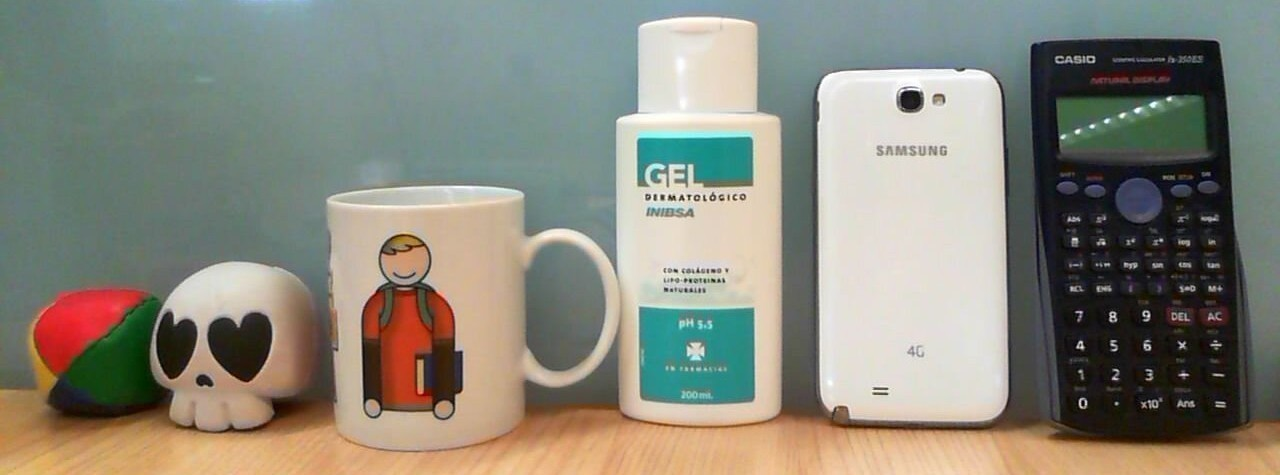
\includegraphics[scale=0.35]{img/tests/dataset.jpg}
				\caption[Experimental dataset]{Experimental dataset}
				\end{center}
		\end{figure}


		Using common objects allow to obtain more reliable experiment results, since they were obtained under working conditions. 
		Common objects are usually featureless. 
		That characteristic complicates the object recognition, since the most textured objects are the ones that usually generate more robust descriptors. 
		In order to overcome this difficulty, different views of each object are obtained and compared when doing the matching. 
		Also, the introduction of both 2D and 3D features diminish the possibilities of false positives and false negatives. 
		\\%[0.5cm]

	% \subsection{Effectiveness measurement}

		% The effectiveness is measured differently for the learning mode than for the recognizing mode. 
		% \\

		% The first mode do not have a possibility of failing in learning, since all the different classes are previously tested and an error on it could only come from a software error. Having this in mind, the effectiveness of this mode is to create the best descriptors possible. 
		% The best descriptor is that one that has a lower size but still is sufficiently robust to allow a good recognition performance. 
		% \\

		% In the case of the second mode, the recognizing, the effectiveness is measured in terms of false negatives and positives versus the true ones. The result is a percentage that indicates how well the features are matched. If the effectiveness is 0\%, the software has a 100\% of false positives and negatives, and if the effectiveness is a 100\%, there is a 100\% of true positives and negatives. 
		% Also, a confusion matrix is constructed using the results of this test in order to offer a visual summary of the performance of the code. 	\\

		% Finally, the F-score or F-measure is computed in order to present the accuracy of the of the system developed in this thesis. 
		\paragraph{Accuracy measurement}\mbox{}\\


		The accuracy of the system is measured using the F-score or F-measure. 
		The general formula for a positive real $\beta$ is the following: 
		\\

		$F_\beta=(1+\beta^2)\cdot\frac{precision \cdot recall}{(\beta^2 \cdot precision )+recall}$
		\\



		
		% The F-score may be expressed in terms of true and false positives and negatives as shown below: 
		% \\

		% $F_\beta=\frac{(1+\beta^2)\cdot true\_positives}{(1+\beta^2)\cdot true\_positives +\beta^2 \cdot false\_negatives +false\_positives}$
		% \\

		The $F_1 score$ is used when the weight of having false positives and negatives is the same. 
		This weight depends on the applications of the system being tested. 
		For example, in critical systems such as a police face recognition software it is preferable to have false positives than false negatives. 
		It is obtained from the general formula for $\beta=1$: 	
		\\

		$F_1=2\cdot\frac{precision \cdot recall}{precision + recall}$
		\\

		In the system there is no difference between both errors and hence the $F_1 score$ is the ratio being used. 
		In order to evaluate the accuracy, a confusion matrix is constructed for each experiment. 
		This matrix shows the number of times each different object was predicted when each of the real objects were presented to the system. 
		In this system, each different retrieved a different number of results and hence the matrix is constructed with a ratio from 0 to 1. 
		The confusion matrix in which the results are being presented is the same as the figure below. 


		\begin{figure}[H]
				\begin{center}
			    \includegraphics[scale=0.35]{img/tests/matrix_model.png}
				\caption[Confusion matrix model]{Confusion matrix model}
				\end{center}
		\end{figure}


		The precision is the fraction of retrieved results that are relevant.  
		Using a confusion matrix as the one above, the precision is computed from it as follows: 
		\\

		$precision_{ij}=\frac{M_{ij}}{\sum M_j}$
		\\

		The recall is the fraction of the results that are relevant and that have succeeded. 
		It may be obtained using the confusion matrix with this formula: 
		\\

		$recall_{ij}=\frac{M_{ij}}{\sum M_i}$
		\\

		The precision and recall is computed for each of the six objects conforming the dataset. 
		Those two parameters together with the F1-score is presented in a table as the one that can be seen below. 

		\begin{figure}[H]
				\begin{center}
			    \includegraphics[scale=0.35]{img/tests/fscore_model.png}
				\caption[F1-score table model]{F1-score table model using precision and recall measurements}
				\end{center}
		\end{figure}

		% Since the experiments retrieve the true and false positives and negatives, the formula that is used is the one below: 
		% \\


		% $F_\beta=\frac{2\cdot true\_positives}{2\cdot true\_positives + false\_negatives +false\_positives}$
		% \\

